\chapter{Явление сверхпроводимости}

\section{Основные характеристики сверхпроводящего состояния}

Согласно теории Гинзбурга-Ландау обычно сверхпроводник вблизи \( T_c \) 
описывается одним комплексным параметром поля. Физика этих систем определяется 
двумя фундаментальными масштабными длинами, глубиной проникновения магнитного 
поля \( \lambda \) и длиной когерентности \( \xi \), а также коэффициентом 
\( \kappa \), который определяет реакцию на внешнее поле, разделяя их на две  
категории следующим образом; сверхпроводники первого рода, где 
\( \kappa < 1/\sqrt{2} \) и второго рода, где \( \kappa > 1/\sqrt{2} \) 
\cite{bib:3}.

Теория БКШ дает исчерпывающее описание сверхпроводящих свойств материала во 
всём температурном интервале от \( 0 \) до \( T_c \), но является сложной с 
математической точки зрения. Поэтому часто физики прибегают к другому, 
относительно более простому способу анализа сверхпроводящего состояния -- 
Теория Гинзбурга–Ландау, которая прекрасно описывает, качественно и 
количественно, поведение сверхпроводника, но работает только в ограниченном 
интервале вблизи критической температуры.

ТГЛ основывается на теории фазовых переходов второго рода. В этой теории, 
наряду с критической температурой, длиной когерентности и лондоновской глубиной 
проникновения, вводится ещё одна характеристика, -- параметр порядка. С 
точностью до некоторого коэффициента пропорциональности можно считать, что 
модуль параметра порядка -- это энергетическая щель в теории БКШ. Параметр 
порядка равен нулю при \( T = T_c \) и принимает максимальное значение, когда 
температура достигла абсолютного нуля. Отметим, что есть и иная трактовка 
физического смысла параметра порядка: квадрат его модуля определяет 
концентрацию куперовских пар. Параметр порядка играет ключевую роль в теории 
Гинзбурга–Ландау. Через него выражается свободная энергия сверхпроводника. 
\cite{bib:net}

Задача о сосуществование сверхпроводящего и магнитного порядков привлекает 
внимание исследователей на протяжение последних десятилетий. Можно выделить 
два основных механизма взаимодействия сверхпроводящего параметра порядка с 
магнитной подсистемой: электромагнитный механизм, когда куперовские пары 
взаимодействуют с магнитным полем индуцированным ферромагнетиком (впервые 
такое взаимодействие было рассмотрено В.~Л.~Гинзбургом в 1956 
\cite{ginzburg}): и обменное взаимодействие магнитных моментов с куперовскими 
парами \cite{buzdin,bulaev}. Если ферромагнетик и сверхпроводник разделены 
тонкой диэлектрической прослойкой, то эффект близости подавлен и единственным 
фактором, определяющим взаимодействие подсистем, является магнитное поле, 
создаваемое неоднородным распределением намагниченности в ферромагнетике.
Впервые смешанное состояние с неполным эффектом Мейсснера--Оксенфельда 
(фаза Шубникова) в сверхпроводниках, находящихся во внешнем магнитном поле, 
было обнаружено группой Л.~В.~Шубникова в 1937 году \cite{shubnikov}. В 1957 
году А.~А.~Абрикосов, основываясь на теории Гинзбурга--Ландау 
\cite{ginzburg-landau}, показал, что в массивных сверхпроводниках второго рода 
внешнее магнитное поле проникает в сверхпроводник в виде нитей магнитного 
потока (вихрей Абрикосова) \cite{abrikosov}, которые можно рассматривать как 
структурную единицу смешанного состояния.

\section{Сверхпроводимость 1-го и 2-го рода}

Несмотря на то что теория Гинзбурга–Ландау является феноменологической, то 
есть она не объясняет причины возникновения явления, которое она описывает, с 
её помощью был получен ряд важных результатов. Применив эту теорию, её авторы 
вычислили поверхностную энергию, возникающую на границе сверхпроводника и 
нормального металла в присутствии внешнего магнитного поля. Оказалось, что 
результат зависит от безразмерной величины, называемой параметром 
Гинзбурга–Ландау \( \kappa \): \( \kappa = \lambda/\xi \) (отношение 
лондоновской глубины проникновения к длине когерентности). Из расчетов 
следовало, что при \( \kappa < 1/\sqrt{2} \) поверхностная энергия оказывается 
положительной. Для сверхпроводника цилиндрической формы, ось которого 
параллельна силовым линиям магнитного поля, данный результат означал, что 
переход в нормальное состояние происходит моментально, как только индукция 
магнитного поля превышает некоторое критическое значение \( B_c \) для данной 
температуры (рисунок~\ref{img:01}). В принципе, ничего нового Гинзбург и 
Ландау не получили, они лишь теоретически подтвердили хорошо известный уже на 
тот момент экспериментальный факт поведения сверхпроводников.

\begin{figure}[h!]
    \center
    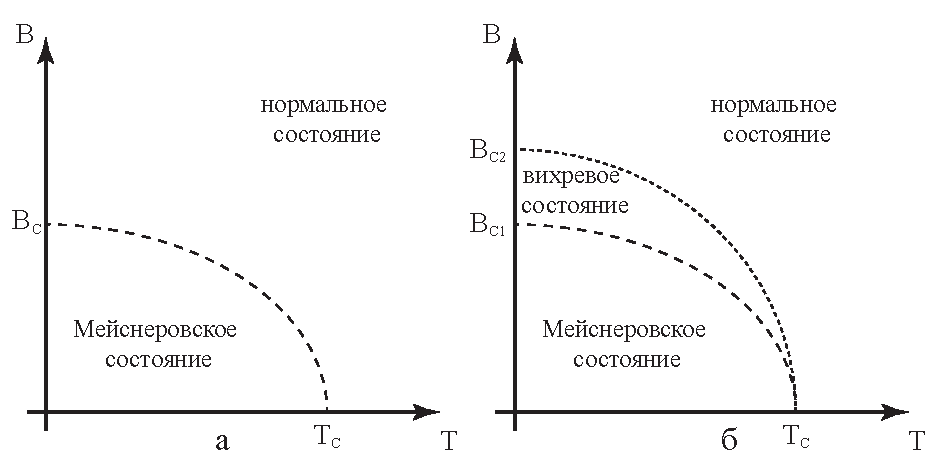
\includegraphics[width=.8\textwidth]{img_01}
    \caption{Фазовая диаграмма состояния сверхпроводников 1-го (а) и 
        2-го (б) рода, показывающая, как меняются состояния сверхпроводника 
        при изменении температуры и индукции внешнего магнитного поля. В 
        мейсснеровском состоянии силовые линии магнитного поля не могут 
        проникнуть в вещество. Смешанное или вихревое состояние означает 
        сосуществование сверхпроводимости и нормальных не сверхпроводящих 
        тонких нитей, вытянутых вдоль линий магнитного поля. Такие нити 
        называют вихрями Абрикосова, или квантовыми вихрями.}
    \label{img:01}
\end{figure}

Советский физик Николай Заварицкий, исследуя тонкие сверхпроводящие плёнки, 
обнаружил, что их поведение в магнитном поле не согласуется с предсказаниями 
теории Гинзбурга–Ландау. Чтобы понять причину расхождения, Алексей Абрикосов, 
основываясь на теории Гинзбурга–Ландау, решил рассмотреть случай, когда 
поверхностная энергия является отрицательной, -- иными словами, попытаться 
понять картину поведения сверхпроводника в магнитном поле с 
\( \kappa > 1/\sqrt{2} \).

Расчёты показали, что пока индукция магнитного поля не превосходит нижнее 
критическое значения поля \( B_{c1} \) при фиксированной температуре, 
сверхпроводник находится в состоянии Мейсснера. После того как индукция 
магнитного поля стала больше \( B_{c1} \), сверхпроводник начинают пронизывать 
своеобразные нити микронных размеров, вытянутые вдоль силовых линий внешнего 
поля. Чем больше индукция поля, тем больше ниток будет в сверхпроводнике. 
Абрикосов установил, что эти образования представляют собой вихри (теперь они 
называются абрикосовскими), ядра которых являются не сверхпроводящими, 
нормальными, с размером порядка длины когерентности \( \xi \), а вокруг них 
протекают циркулирующие сверхпроводящие токи, которые экранируют нормальную 
область вихря (ширина области экранировки равна лондоновской глубине 
проникновения \( \lambda \)). Кроме того, в ходе вычислений обнаружилось, что 
вихри несут в себе как бы одну силовую линию внешнего магнитного поля, или 
квант магнитного потока, флюксоид 
\( \Phi_0 = hc/2e \simeq 2.07\cdot10^{-7} \text{ Гс}\cdot\text{см}^2 \). Вихри 
формируют в сверхпроводнике треугольную решётку, образуя смешанное (оно же 
вихревое) состояние (рисунок~\ref{img:01}).

Если при заданной температуре продолжить усиливать магнитное поле, то при 
верхнем критическом значении \( B_{c2} \) вихрей станет настолько много, что 
их ядра начнут перекрываться, и они заполнят весь объем сверхпроводника, 
переводя его в нормальное состояние (рисунок~\ref{img:01}). \cite{bib:net}

В сверхпроводниках второго рода для того чтобы напряжённость внешнего 
магнитного поля, необходимая для образования вихревых возбуждений, была 
энергетически выгодной, нужно чтобы \( B_{c1} \) было меньше, чем 
термодинамическое значение магнитного поля \( B_{ct} \) (поле, энергетическая 
плотность которого равна энергии конденсации сверхпроводника, т.е. 
сверхпроводящее состояние становится термодинамически неустойчивым); В 
сверхпроводниках первого рода напряжённость поля требует создание вихревого 
возбуждения больше, чем критическое термодинамическое значение магнитного 
поля, т.е. вихри не могут образовываться. Можно выделить также специальный 
<<нульмерный>> пограничный случай, когда \( \kappa \) имеет критическое 
значение точно на границе первого/второго рода, что в самом общей модели ГЛ 
соответствует \( \kappa = 1/\sqrt{2} \). В этом случае вихри не 
взаимодействуют в теории Гинзбурга-Ландау.

В двущелевых сверхпроводниках второго рода сверхпроводящие компоненты 
происходят из электронного куперовского спаривания в различных зонах 
\cite{bib:6}. Поэтому эти конденсаты не могут быть независимо сохраняющимися.

В случае сверхпроводников первого рода две сверхпроводящие компоненты были 
предсказаны, происходящие из электронного и протонного куперовского спаривания 
в атомарном водороде или богатых водородом сплавов. В прогнозируемом 
жидкометаллическом дейтерии и сплавов богатых дейтерием, было предсказано 
существование электронной проводимости на сверхвысоких давлениях с дейтронной 
конденсацией  \cite{bib:12.1,bib:12.2,bib:13,bib:14}. Поскольку электроны не 
могут быть преобразованы в протон или дейтрон с независимо сохраняющейся 
конденсацией, и, следовательно, в эффективной модели Джозефсона 
межкомпонентная связь запрещена на основаниях симметрии. Этот эффект в 
настоящее время является предметом возобновлённых экспериментальных 
исследований.

Это большое разнообразие систем вызывает необходимость истолковать и 
классифицировать возможные магнитные отклики многокомпонентных 
сверхпроводников. В различных источниках обсуждалось, что в многокомпонентных 
системах, где магнитный отклик гораздо сложнее, чем в обычных системах, что 
разделение на сверхпроводники первого/второго рода не является достаточным для 
классификации. Скорее всего существует отдельный сверхпроводящий режим, при 
котором вихри имеют дальнодействующее притяжение, близкодействующее 
отталкивание и образование вихревых узлов в области двухкомпонентного эффекта 
Мейсснера \cite{bib:1,bib:2}. Последние экспериментальные работы 
\cite{bib:16,bib:17} выдвинули предположение, что это состояние реализуется в 
двущелевом материале \( MgB_2 \), что вызвало растущий интерес к этой теме. В 
частности были подняты вопросы по поводу того, что сверхпроводимость типа 1,5 
(как это было названо Мощалковым и другими в \cite{bib:16}) возможна даже в 
случае различных неисчезающих связей (например, внутренняя джозефсоновская 
связь, связь смешанных градиентов и т.д.) сверхпроводящими компонентами в 
разных диапазонах. \cite{bib:main}

\section{Сверхпроводимость 1,5-го рода и двущелевые сверхпроводники}

В 2001 году в дибориде магния \( MgB_2 \) была открыта сверхпроводимость с 
неожиданно высокой критической температурой 39 К. Применяя различные 
экспериментальные техники, учёные установили, что большое значение \( T_c \) 
достигается за счёт наличия в \( MgB_2 \) не одной энергетической щели, а 
двух. То есть в сверхпроводящем дибориде магния присутствует как бы два сорта 
куперовских пар. Их взаимодействие и обеспечивает высокую \( T_c \). Важно 
отметить, что у каждого сорта электронных пар есть свой размер, или своя длина 
когерентности. При этом диборид магния имеет лишь одну величину лондоновской 
глубины проникновения. \cite{bib:net}

Каждой из двух энергетических щелей \( \Delta_1 \) и \( \Delta_2 \) 
соответствует своя длина когерентности \( \xi_1 \), \( \xi_2 \) и лондоновская 
глубина проникновения \( \lambda_1 \), \( \lambda_2 \). Если применить 
критерий Абрикосова для \( MgB_2 \), то получится, что для первой щели 
\( \kappa = \lambda_1 / \xi_1 \approx 0,66 < 1/\sqrt{2} \), а для второй -- 
\( \kappa = \lambda_2 / \xi_2 \approx 3,68 > 1/\sqrt{2} \). Получается, что в 
дибориде магния одновременно <<живут>> две сверхпроводимости -- первого и 
второго рода.

В 2003 году в журнале <<Physical Review B>> появилась статья учёных из России, 
Швейцарии и США <<Vortex structure in \( MgB_2 \) single crystals observed by 
the Bitter decoration technique>>, в которой они сообщали о наблюдении 
абрикосовской решётки в чистом монокристалле \( MgB_2 \) в слабом магнитном 
поле. Эксперимент показал, что диборид магния, несмотря на наличие в нем двух 
энергетических щелей, можно отнести к сверхпроводникам второго рода. 
Результат подтверждался снимком треугольной вихревой решётки. Вихри 
распределены равномерно -- что, по мнению исследователей, доказывает факт 
наличия в \( MgB_2 \) сверхпроводимости второго рода.

\begin{figure}[h!]
    \center
    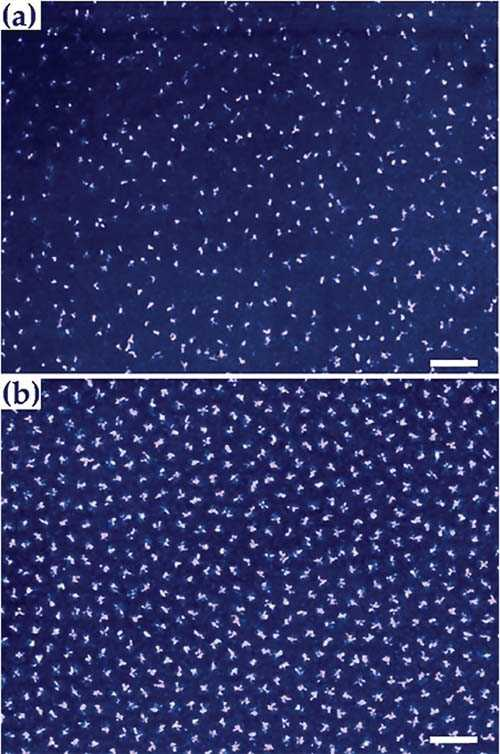
\includegraphics[width=.6\textwidth]{img_spc}
    \caption{Изображения вихревых структур в сверхпроводниках при 
        \( T = 4,2 K \) во внешнем магнитном поле напряжённостью 1 эрстед.
        Вихри в монокристалле \( MgB_2 \) (a) распределены неравномерно, тогда 
        как в монокристалле \( NbSe_2 \) (b) они образуют абрикосовскую 
        треугольную решётку. Длина масштабной линейки 10 мкм.}
    \label{img:spc}
\end{figure}

Однако относительно недавно группа исследователей из Бельгии и Швейцарии 
опубликовала в Архиве препринтов результаты своего эксперимента под говорящим 
заголовком <<Type-1.5 Superconductors>>. Во внешнем магнитном поле 
напряжённостью 1 эрстед (в 4 раза слабее, чем в эксперименте 2003 года) они 
получили для сверхпроводящего чистого монокристалла диборида магния необычную 
картину вихревой решётки -- с неравномерным распределением вихрей 
(рисунок~\ref{img:spc}а). Эта нерегулярность связана с тем, что, как 
предсказывает теория, взаимодействие магнитных вихрей должно напоминать 
поведение межмолекулярных сил: на близких расстояниях вихревые структуры 
отталкиваются, на далёких -- начинают притягиваться. Такое поведение вихрей 
авторы статьи считают главной особенностью сверхпроводимости <<полуторного>> 
рода. \cite{bib:superconductors}

Возможность нового типа сверхпроводимости, отличного от первого и второго рода 
в многокомпонентных системах \cite{bib:1,bib:2} основана на следующих 
соображениях. Краевая задача уравнения Гинзбурга-Ландау в присутствии 
циркуляции фазы сводится к одномерной задачи в целом. Кроме того, как указано в 
\cite{bib:1,bib:2}, в общей двухкомпонентной модели есть три фундаментальные 
масштабные длины, которые указывают на невозможность параметризовать модель с 
точки зрения одного безразмерного параметра \( \kappa \). В случае, когда 
конденсаты не связаны межзонной джозефсоновской связью, при условии, что 
векторный потенциал этих масштабных длин представлен двумя независимыми 
величинами: длиной когерентности и глубиной проникновения магнитного поля. В 
противоположность этому, в случае, когда конденсаты объединяются межзонными 
джозефсоновскими условиями, можно не увидеть различий между длинами 
когерентности и отнести их к различным конденсатам. Тем не менее, в этом 
случае колебания плотности также могут обладать двумя основными 
пространственными длинами \cite{bib:2}, в отличие от однокомпонентных теорий. 
В \cite{bib:1,bib:2} вихревых решениях в двухкомпонентной теории были найдены 
компоненты, которые имеют немонотонное вихревое взаимодействие, с 
доминирующими частями отвечающие за дальнодействующее взаимодействие, 
отталкивающей частью близкодействия и частью отвечающею за электромагнитное 
взаимодействие. Важным обстоятельством, которое было продемонстрировано, 
является то, что эти вихри термодинамически стабильны, несмотря на 
существование притягивающего хвоста во взаимодействии.

\begin{figure}[h!]
    \center
    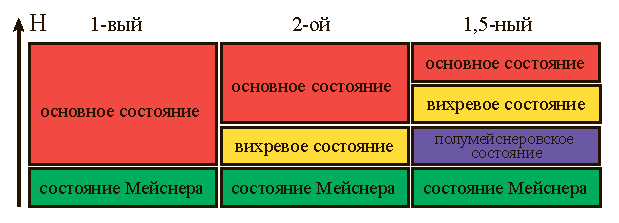
\includegraphics[width=.8\textwidth]{1-01}
    \caption{Сравнение фазовых диаграмм магнитных фаз чистых сверхпроводников
        первого, второго и полуторного рода при нулевой температуре. В 
        полумейсснеровском режиме макроскопическое разделение фаз в 
        двухкомпонентном состоянии Мейсснера и вихревых скоплений, где 
        один из режимов плотности подавляется внутренним перекрытием.}
    \label{fig:1}
\end{figure}

Немонотонный межвихревой потенциал взаимодействия должен привести к 
образованию вихревых скоплений в слабомагнитном поле, погруженного в 
безвихревую область, эффект упомянутый в \cite{bib:1} как 
<<полумейсснеровское состояние>>. На рисунке~\ref{fig:1} схематически 
показана фазовая диаграмма сверхпроводника 1,5-го рода.

Если вихри образуют кластеры, то нельзя использовать обычный одномерный 
аргумент относительно энергии сверхпроводника в нормальном состоянии границы 
раздела для классификации магнитного отклика системы. Прежде всего, энергия 
на вихрь, в таком случае, зависит от того, находится ли вихрь в кластере или 
нет: т.е. формирование единого изолированного вихря может быть энергетически 
невыгодным, в то время как формирование вихревых кластеров выгодно, потому что 
в кластере, где помещены вихри, создаётся минимум потенциала взаимодействия, 
энергия на квант потока меньше, чем для изолированного вихря (термодинамически 
немонотонный потенциал взаимодействия двух вихрей предусматривает, что 
наименьшей энергией, на квант потока, будет в случае равномерной сетки с шагом 
равным минимуму межвихревого потенциала двух тел).

Таким образом, помимо энергии вихря в кластере, появляется дополнительная 
энергическая характеристика, связанная с границей кластера. Другими словами, в 
этой ситуации, для определения магнитного отклика системы недостаточно 
изучения краевой задачи и задачи одиночного вихря, в отличии от системы 
отдельных составляющих. В кластере система стремится к минимуму граничной 
энергии (так же, как и в сверхпроводниках 1-го рода), в то время нарушение 
структуры одноквантового вихря внутри кластера (аналогично сверхпроводимости 
второго рода с отрицательной энергией межфазного взаимодействия). Таким 
образом, увеличение магнитного поля происходит посредством фазового перехода 
первого рода. Магнитная фаза отлична от вихря в состоянии Мейсснера, затем 
возникает макроскопическое фазовое распределение в двухкомпонентной области 
Мейсснера и вихревых кластерах, где один из режимов подавляется основным 
перекрытием. \cite{bib:main}

\newpage